%!TEX root = ../report.tex
\section{Hopf bifurcation}

Continuing on the upper branch of the pitchfork, we compute (at most) 6 of the eigenvalues closest to the origin after a few steps in $Re.$ After a while we find that a conjugate eigenpair crosses the imaginary axis, which indicates a Hopf bifurcation is nearby. The movement of the eigenvalues is visualized in Figure~\ref{fig:eigenpair_crossing_imag}.

\begin{figure}[h]
  \centerline{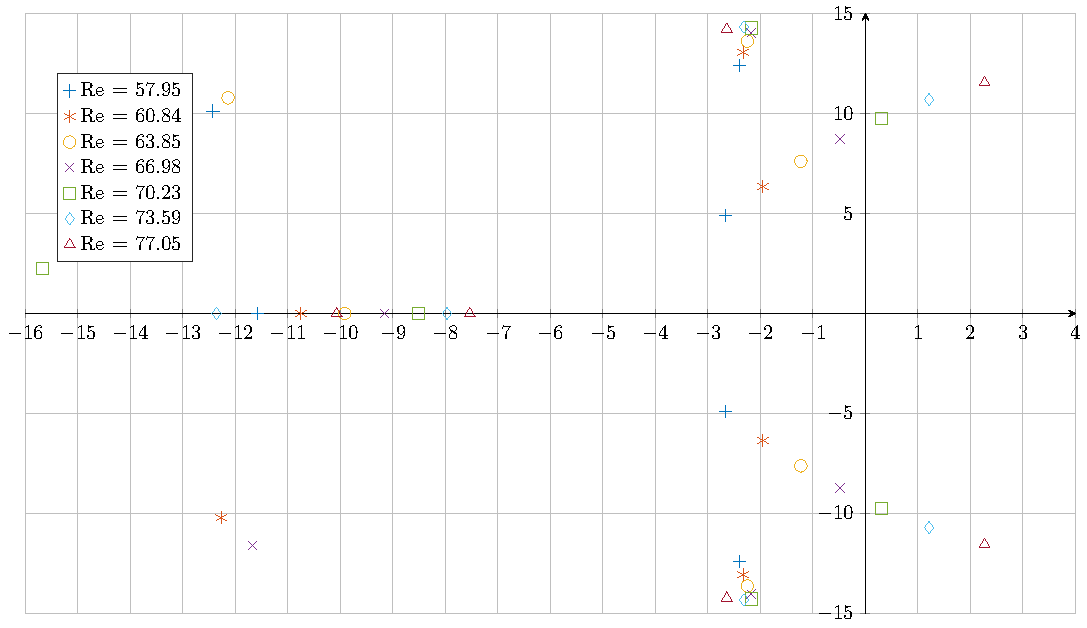
\includegraphics{images/eigenwaarden_hopf.pdf}}
  \caption{A conjugate eigenpair crossing the imaginary axis.}
  \label{fig:eigenpair_crossing_imag}
\end{figure}

We apply the secant procedure to compute the value of $Re$ where the first eigenvalue $\lambda$ is completely imaginary, i.e. $\Re(\lambda) = 0.$ We find that the Hopf bifurcation is located at $Re_H \approx 68.9781.$ The conjugate eigenpair is $$\lambda_\pm \approx \pm 9.372i.$$

Lastly we are interested in the corresponding eigenvectors. In fact they consist of two parts, since there are two discretized unknowns $\psi$ and $\zeta.$ The idea is to reconsider the eigenvalue problem of Equation~\eqref{eq:eigs} and interpret the Jacobian as being of the form
\begin{equation}
    DF_{\*u} = [DF_{\*\psi}, DF_{\*\zeta}]
\end{equation}
so that the first part of an eigenvector corresponds to the eigenfunction of $\psi$ and the second half of it corresponds to the eigenfunction of $\zeta.$ Also, we have both a real and an imaginary part of the eigenfunction. In Figure~\ref{fig:eigenfunction} we have plotted the ones corresponding to $\lambda_+.$ Note that the eigenfunction of $\lambda_-$ is identical up to a sign flip in the complex part.

\begin{figure}[h]
    \centering
    \caption{Eigenfunctions corresponding to $\lambda \approx 9.372i$.}\label{fig:eigenfunction}
    \centerline{
    \begin{subfigure}[b]{0.6\textwidth}
        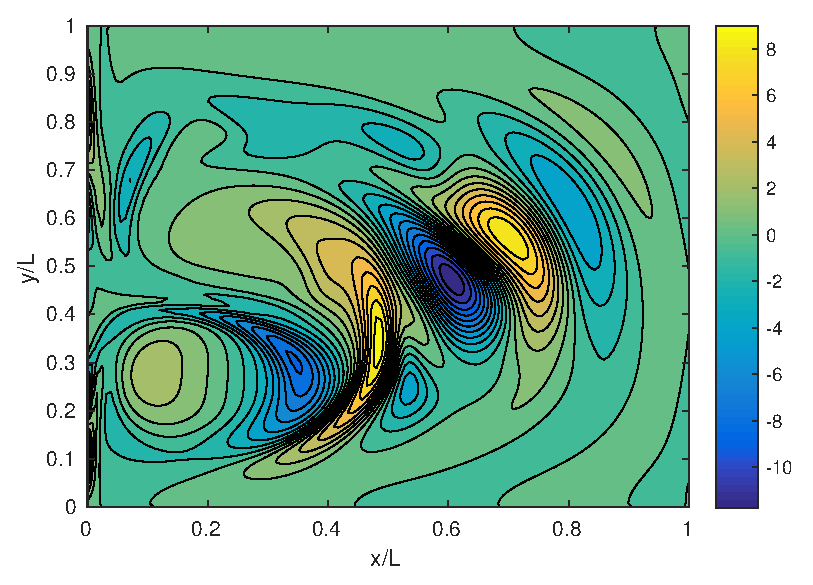
\includegraphics[width=\textwidth]{images/eigenvector_hop_1_2.eps}
        \caption{Real part corresponding to $\psi$}
        \label{fig:real_psi}
    \end{subfigure}
    ~
    \begin{subfigure}[b]{0.6\textwidth}
        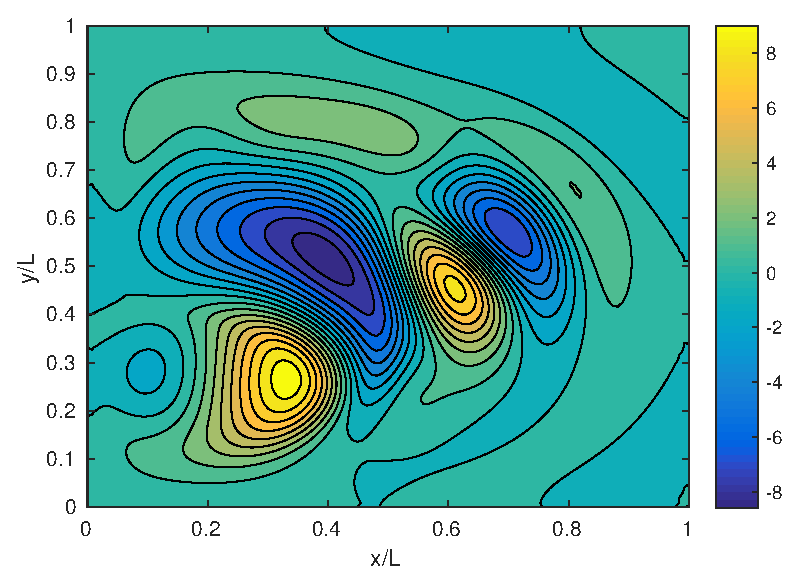
\includegraphics[width=\textwidth]{images/eigenvector_hop_2_2.eps}
        \caption{Real part corresponding to $\zeta$}
        \label{fig:real_zeta}
    \end{subfigure}
    }
    \centerline{
    \begin{subfigure}[b]{0.6\textwidth}
        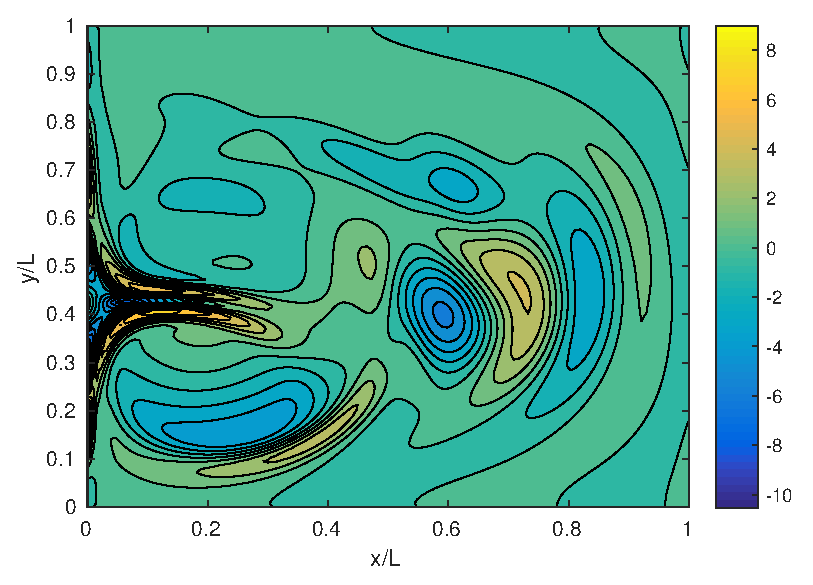
\includegraphics[width=\textwidth]{images/eigenvector_hop_1_3.eps}
        \caption{Imaginary part corresponding to $\psi$}
        \label{fig:imag_psi}
    \end{subfigure}
    ~
    \begin{subfigure}[b]{0.6\textwidth}
        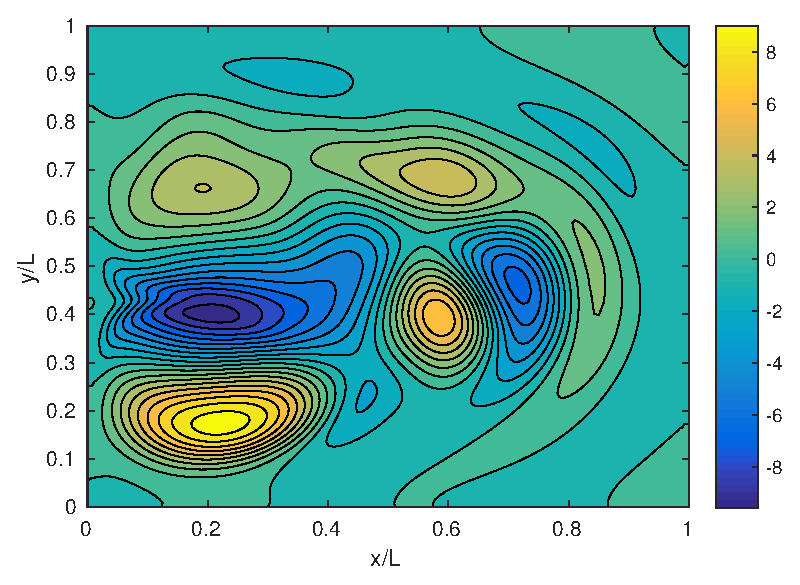
\includegraphics[width=\textwidth]{images/eigenvector_hop_2_3.eps}
        \caption{Imaginary part corresponding to $\zeta$}
        \label{fig:imag_zeta}
    \end{subfigure}
    }
\end{figure}